\newpage

\section{Разработка архитектурно-структурных решений}

Выполнение кода предметно-ориентированного языка осуществляется за счет интерпретатора,
который должен быть спроектирован в виде модуля, подключаемого к серверной части конструктора Telegram ботов.

Обобщенная модульная структура серверной части конструктора представлена на рисунке~\ref{f:modules_server_struct}.

\begin{figure}[ht]
	\centering
	\vspace{\toppaddingoffigure}
	% 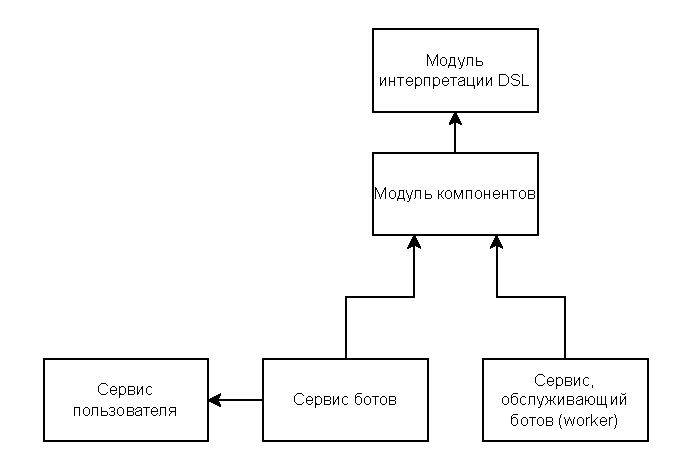
\includegraphics[width=0.7\textwidth]{structures/modules_server_struct.pdf}
	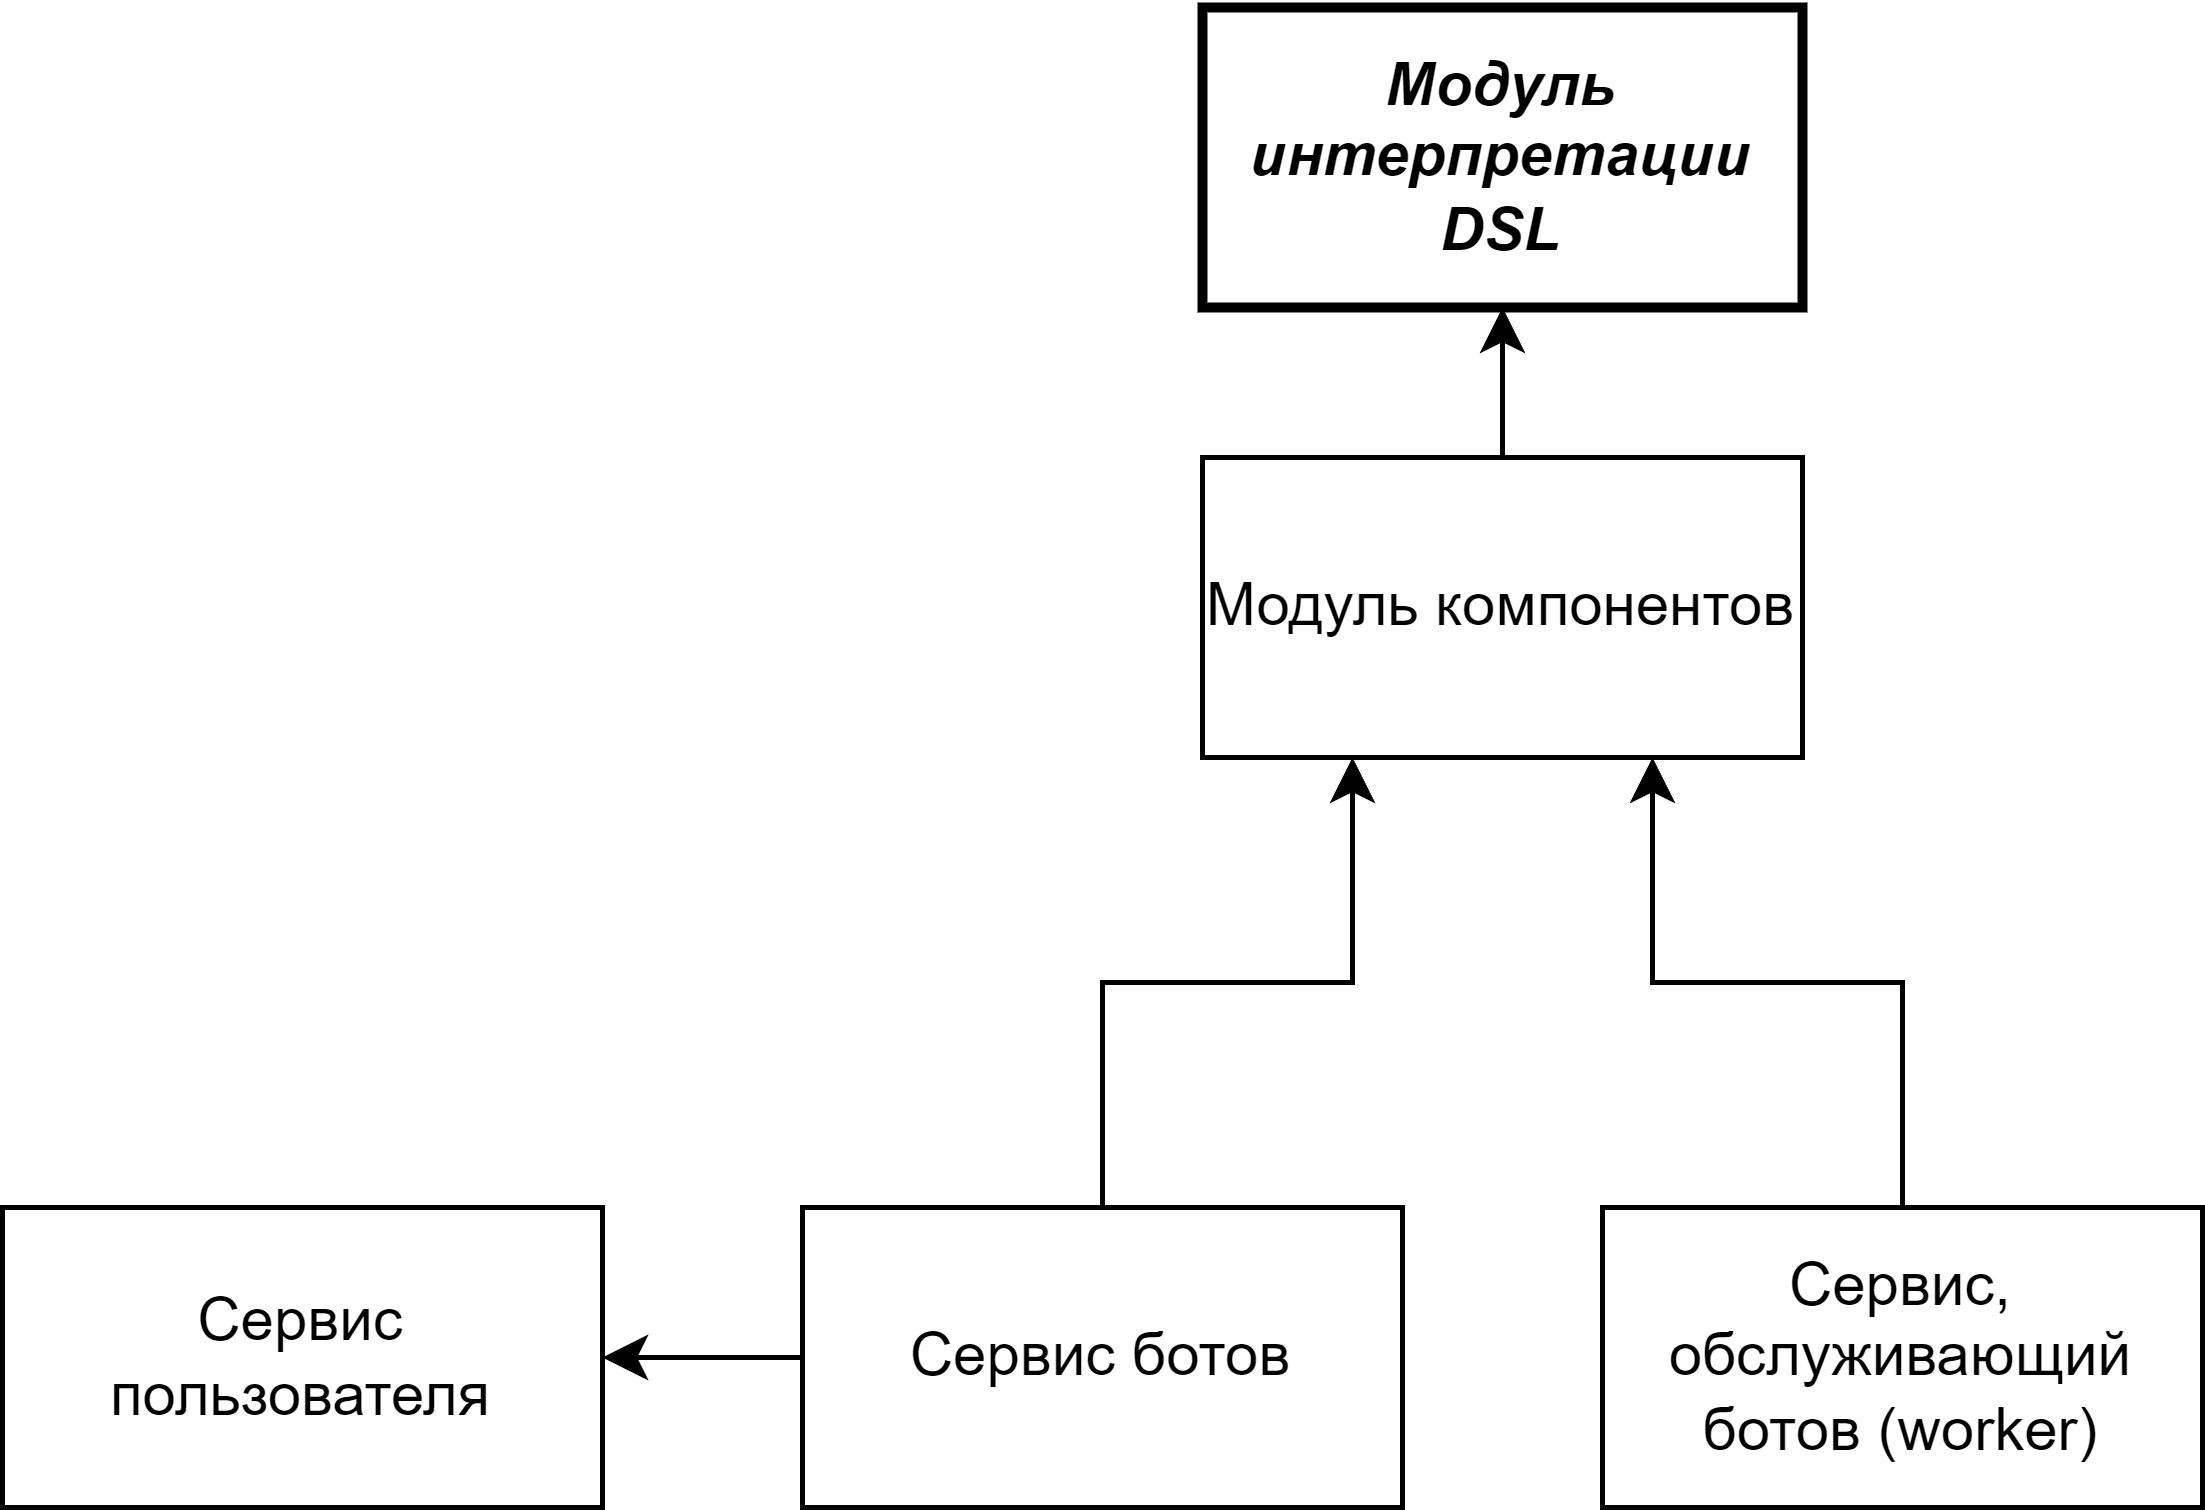
\includegraphics[width=0.7\textwidth]{structures/modules_server_struct.png}
	\caption{Модульная структура серверной части конструктора}
	\label{f:modules_server_struct}
\end{figure}

Сервис ботов отвечает за управление состоянием бота и редактирование его компонентной структуры.
Сервис ботов зависит от сервиса пользователей, который предоставляет первому методы для авторизации пользователя.
Также сервис ботов зависит от модуля компонентов, который описывает структуры компонентов и реализует их логику выполнения.

Обслуживающий сервис отвечает за логику работы бота. 
Он выполняет обработку запроса к боту от пользователя Telegram.
В соответствии с разработанной компонентной структурой бота, обслуживающий сервис вызывает методы модуля компонентов для запуска их логики выполнения.

Одним из компонентов является компонент выполнения кода на предметно-ориентированном языке.
Отсюда, модуль компонентов зависит от модуля интерпретации предметно-ориентированного языка.
При запуске компонента выполнения DSL кода, выполняется вызов функции выполнения кода из модуля интерпретации.

В данном проекте для возможности интеграции с серверной частью конструктора Telegram ботов необходимо реализовать программный интерфейс,
который бы предоставлял возможность передачи кода и значений внешних переменных, интерпретатору предметно-ориентированного языка.

Работа интерпретатора состоит из последовательного выполнения следующих этапов:
\begin{enumerate}
	\item лексический анализ;
	\item синтаксический анализ;
	\item семантический анализ;
	\item исполнение команд.
\end{enumerate}

Обобщенная структура интерпретатора представлена на рисунке~\ref{f:full_interpreter_struct}.

\begin{figure}[ht]
	\centering
	\vspace{\toppaddingoffigure}
	% 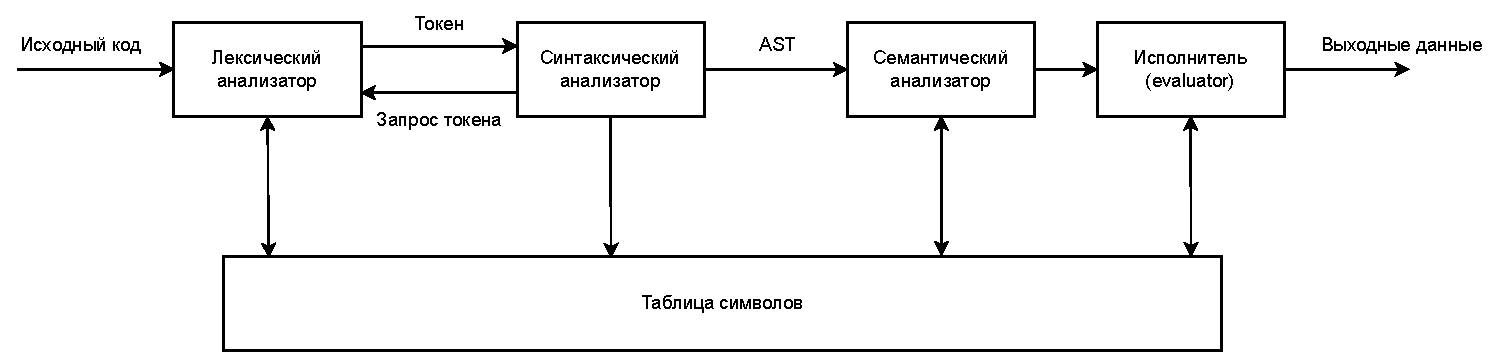
\includegraphics[width=1.0\textwidth]{structures/full_interpreter_struct.pdf}
	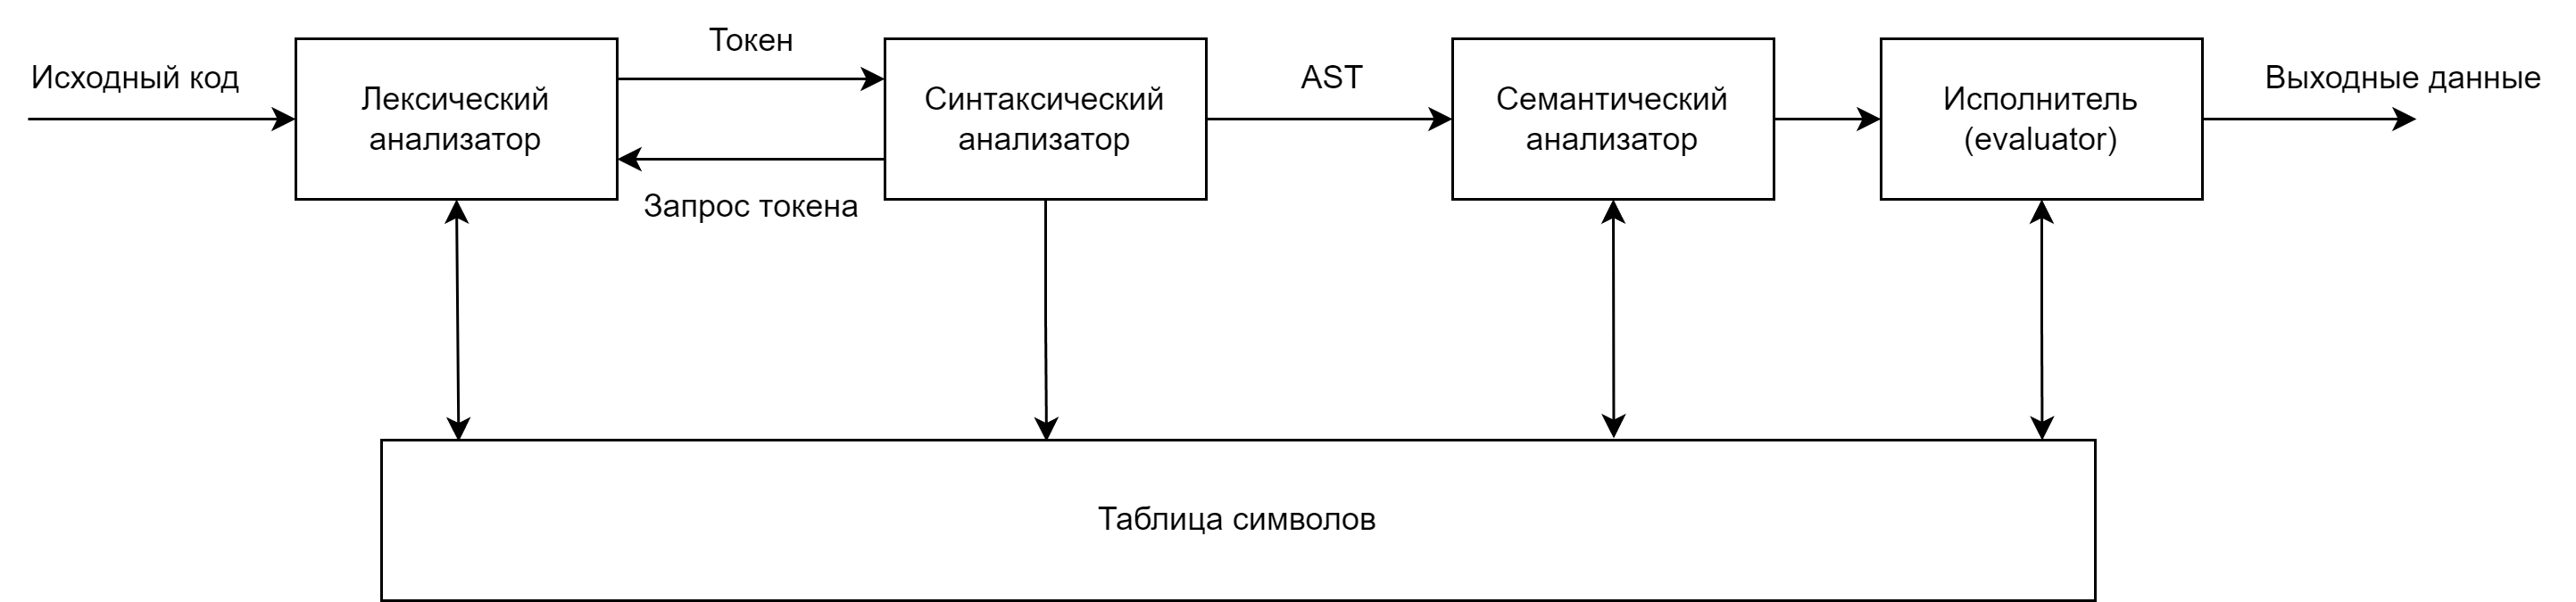
\includegraphics[width=1.0\textwidth]{structures/full_interpreter_struct.png}
	\caption{Обобщенная структура интерпретатора}
	\label{f:full_interpreter_struct}
\end{figure}

Для решения поставленной задачи, в первую очередь, необходимо в соответствии с указанными требованиями
разработать грамматику предметно-ориентированного языка и спроектировать обобщенную структуру программы интерпретатора.

\subsection{Разработка грамматики языка}

Описание языка программирования основывается на теории формальных языков.
В данном разделе проводится разработка формальной грамматики языка и её описание.


\subsubsection{Способы задания языков}

Для задания языка можно воспользоваться следующими методами:

\begin{enumerate}
    \item перечислить все цепочки языка;
    \item указать способ порождения цепочек;
    \item определить метод распознавания допустимых цепочек.
\end{enumerate}

Перечисление всех цепочек языка возможно в исключительных случаях, например,
когда для управления некоторой системой достаточно двух-трех команд.

Механизм порождения цепочек предполагает использование формальной порождающей грамматики.

Формальная порождающая грамматика -- это математическая система, описывающая правила построения цепочек некоторого (формального) языка \refref{ref:grammar}.

Распознавание допустимых цепочек осуществляется с помощью некоторого логического устройства -- распознавателя.
На вход распознавателя подается цепочка, а на выходе образуется логическое значение <<истина>> в случае принадлежности цепочки языку
и <<ложь>>, если цепочка языку не принадлежит.
Распознаватели строятся на основе теорий конечных автоматов и автоматов с магазинной памятью.

Методы порождения и распознавания тесно связаны.
Механизм порождения обычно используется при описании языка, а распознаватель при его реализации, т.е. в трансляторе.

Описать синтаксис языков программирования можно несколькими способами, например, такими как формы Бэкуса-Наура, диаграммы Вирта и другими.
Это методы задают правила вывода, определяющие возможные конструкции цепочек языка.
В данном проекте для описания грамматики языка используется расширенная форма Бэкуса-Наура (РБНФ).



\subsubsection{Применение расширенной формы Бэкуса-Наура для описания формальной грамматики языка}

Расширенная форма Бэкуса-Наура – формальная система определения синтаксиса,
в которой одни синтаксические категории последовательно определяются через другие.
Используется для описания контекстно-свободных грамматик \refref{ref:rbnf}.

Формальная грамматика задаётся четвёркой вида:

\(G = (V_T, V_N, P, S)\),

где \(V_T\) -- множество терминальных символов грамматики – конечные
элементы языка, не разбирающиеся на более мелкие составляющие в рамках
синтаксического анализа, например ключевые слова, цифры, буквы
латинского алфавита.

\(V_N\) -- конечное множество нетерминальных символов – элементов грамматики, имеющих собственные имена и структуру.
Каждый нетерминальный символ состоит из одного или более терминальных и/или нетерминальных символов.

\(P\) -- множество правил вывода грамматики.

\(S\) -- начальный символ грамматики, \(S \in V_N\) \refref{ref:grammar}.

РБНФ является одним из способов представления формальных грамматик.
РБНФ состоит из множества правил вывода, каждое из которых определяет синтаксис некоторой конструкции языка.

Некоторые основные конструкции РБНФ:

\begin{itemize}
    \item A, B -- конкатенация элементов;
    \item A | B -- выбор (A или B);
    \item {[A]} -- элемент в квадратных скобках может отсутствовать (аналог - <<?>>);
    \item \{A\} -- повторение элемента 0 или более раз (аналог - <<*>>);
    \item (A B) -- группировка элементов;
    \item (* … *) – комментарий;
    \item <<;>> – отмечает окончание правила (аналог - <<.>>).
\end{itemize}

Кроме того, в качестве синтаксического сахара могут использоваться следующие символы:

\begin{itemize}
    \item <<*>> - предыдущий элемент может встречаться 0 или более раз;
    \item <<?>> - предыдущий элемент является необязательным (присутствует 0 или 1 раз);
    \item <<+>> - предыдущий элемент встречается 1 или более раз.
\end{itemize}

В соответствии с данными правилами описание синтаксиса предметно-ориентированного языка будет выглядеть следующим образом:

(* Точка входа *)

Program = Statement+ \\


(* Основные конструкции *)

Statement = AssignStmt | FunctionDecl | ExpressionStmt | ReturnStmt | BlockStmt | IfStmt .

ExpressionStmt = Expression . \\

AssignStmt = Identifier assign\_op Expression .

ReturnStmt = "{}return"{} [Expression] .

BlockStmt = "{}\{"{} StatementList "{}\}" .

StatementList = \{ Statement "{};"{} \} .

IfStmt = "{}if("{} [Expression] "{})"{} BlockStmt ["{}else"{} BlockStmt] . \\


(* Выражения *)

Expression = UnaryExpr | Expression binary\_op Expression . 

UnaryExpr = PrimaryExpr | unary\_op UnaryExpr . \\

PrimaryExpr = Operand | PrimaryExpr Index | CallExpr .

Index = "{}["{} Expression "{}]"{} .

ExpressionList = Expression \{ "{},"{} Expression \} . \\


(* Определение структуры функции *)

FunctionDecl = "{}fn("{} [ParameterList] "{})"{} BlockStmt .

ParameterList = Identifier \{ "{},"{} Identifier \} .

Arguments = "{}("{} [ ExpressionList ] "{})"{} .

CallExpr = Identifier Arguments . \\


(* Массив *)

Array = "{}["{} [ ExpressionList ] "{}]"{} . \\


(* Хэш-карта *)

Key = stringLiteral | intLiteral | Identifier | Expression .

KeyedElement  = [ Key "{}:"{} Expression ] .

Map = "{}\{"{} KeyedElement \{ "{},"{} KeyedElement \} "{}\}"{} . \\


Identifier = (letter | "{}\_"{}) { letter | "{}\_"{} | digit } .

Operand = Literal | "{}("{} Expression "{})"{} .

Literal = intLiteral | stringLiteral | Array | Map .

intLiteral = digit \{ digit \} .

stringLiteral = << "{} >> \{ ascii\_char \} << "{} >> . \\


(* Операторы *)

binary\_op = "{}||"{} | "{}\&\&"{} | rel\_op | add\_op | mul\_op .

rel\_op = "{}=="{} | "{}!="{} | \"{}<\"{} | "{}<="{} | "{}>"{} | "{}>="{} .

add\_op = "{}+"{} | "{}-"{} .

mul\_op = "{}*"{} | "{}/"{} | "{}\%"{} .

assign\_op = "{}="{} .

unary\_op = "{}-"{} | "{}!"{} . \\


(* Примитивы (цифры, буквы) *)

digit = "{}0"{} ... "{}9"{} .

letter = "{}A"{} ... "{}Z"{} | "{}a"{} ... "{}z"{} .

ascii\_char = ascii character . \\

Начальное состояние, с которого начинается разбор -- Program.

% В данном разделе была разработана и описана с помощью расширенной формы Бэкуса-Наура формальная грамматика предметно-ориентированного языка.
\subsection{Разработка лексического анализатора}

% В данном разделе необходимо выполнить разработку алгоритмов функционирования лексического анализатора.

Лексический анализ – процесс разбора входной последовательности символов на распознанные группы – лексемы.

Лексемой является структурная (минимальная значимая) единица языка, состоящая из элементарных символов языка и не содержащая в своём составе других структурных единиц языка.

В ходе выполнения лексического анализатора каждая лексема идентифицируется и преобразуется в токен.

Токен – экземпляр лексемы, представляющий собой пару «тип лексемы» и «значение».
«Тип» указывает на принадлежность лексемы к определенной категории, например, идентификатор, число и т.д., а «значение» содержит конкретные данные, соответствующие этой лексеме.

Категории токенов, которые используются в разрабатываемом предметно-ориентированном языке:
\begin{itemize}
    \item идентификаторы;
    \item числа;
    \item строки;
    \item разделители;
    \item операторы (арифметические, сравнения и т.д);
    \item скобки;
    \item специальные (конец входной последовательности и т.п)
    \item ключевые слова.
\end{itemize}

Полный список токенов с указанием категории и примерами лексем приведен в таблице~\ref{t:tokens}.

Процесс лексического анализа является первым шагов в трансляции исходного кода программы и формирует основу для следующих этапов,
таких как синтаксический анализ и построение абстрактного синтаксического дерева.

\clearpage

\begin{table}[h!]
    \Large
    \centering
    \begin{threeparttable}
        \caption{Токены с примерами}
        \label{t:tokens}
        \begin{tabularx}{\textwidth}{|X|c|c|}
            \hline
            Токен         & Категория      & Пример лексемы  \\
            \hline
            IDENT         & Идентификатор  & qwe             \\
            \hline
            INT           & Число          & 123             \\
            \hline
            STRING        & Строка         & «привет, hello» \\
            \hline
            ASSIGN        & Оператор       & =               \\
            \hline
            PLUS          & Оператор       & +               \\
            \hline
            MINUS         & Оператор       & -               \\
            \hline
            STAR          & Оператор       & *               \\
            \hline
            SLASH         & Оператор       & /               \\
            \hline
            EXCLAMINATION & Оператор       & !               \\
            \hline
            PERCENT       & Оператор       & \%              \\
            \hline
            EQ            & Оператор       & ==              \\
            \hline
            NEQ           & Оператор       & !=              \\
            \hline
            LEQ           & Оператор       & <=              \\
            \hline
            GEQ           & Оператор       & =>              \\
            \hline
            LT            & Оператор       & <               \\
            \hline
            GT            & Оператор       & >               \\
            \hline
            LAND          & Оператор       & \&\&            \\
            \hline
            LOR           & Оператор       & ||              \\
            \hline
            COMMA         & Разделитель    & ,               \\
            \hline
            SEMICOLON     & Разделитель    & ;               \\
            \hline
            LPAR          & Скобка         & (               \\
            \hline
            RPAR          & Скобка         & )               \\
            \hline
            LBRACE        & Скобка         & \{              \\
            \hline
            RBRACE        & Скобка         & \}              \\
            \hline
            LBRACKET      & Скобка         & [               \\
            \hline
            RBRACKET      & Скобка         & ]               \\
            \hline
            IF            & Ключевое слово & if              \\
            \hline
            ELSE          & Ключевое слово & else            \\
            \hline
            TRUE          & Ключевое слово & true            \\
            \hline
            FALSE         & Ключевое слово & false           \\
            \hline
            FUNC          & Ключевое слово & fn              \\
            \hline
            RETURN        & Ключевое слово & return          \\
            \hline
            ILLEGAL       & Специальный    & @               \\
            \hline
            EOF           & Специальный    & Конец файла     \\
            \hline
        \end{tabularx}
    \end{threeparttable}
    \vspace{\bottompaddingoftable}
\end{table}

Схема взаимодействия лексического и синтаксического анализаторов показана на рисунке~\ref{f:la_sa_struct}.

\begin{figure}[ht]
	\centering
	\vspace{\toppaddingoffigure}
	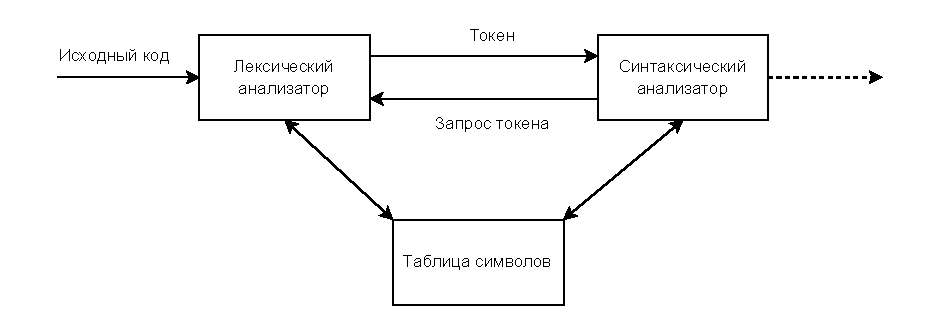
\includegraphics[width=0.9\textwidth]{structures/lexical_analyzer/la_sa_struct.pdf}
	\caption{Схема взаимодействия лексического и синтаксического анализаторов}
	\label{f:la_sa_struct}
\end{figure}

При запросе нового токена лексический анализатор считывает входной поток символов до точной идентификации следующего токена.

Процесс распознавания токенов из входного потока символов языка можно показать с помощью диаграмм переходов состояний.

На рисунке~\ref{f:dps_eq_assign} показана диаграмма для определения токенов «=» и «==».

\begin{figure}[ht]
	\centering
	\vspace{\toppaddingoffigure}
	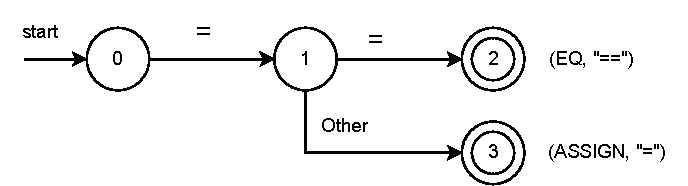
\includegraphics[width=0.9\textwidth]{structures/lexical_analyzer/dps_eq_assign.pdf}
	\caption{Диаграмма переходов для определения «=» и «==»}
	\label{f:dps_eq_assign}
\end{figure}

Работа начинается с состояния 0, в котором считывается следующий символ из входного потока.
Если полученный символ «=», то по дуге, помеченной «=» выполняется переход в состояние 1.
В состоянии 1 выполняется считывание следующего символа.
Если этот символ «=», выполняется переход в состояние 2 – заключительное состояние,
в котором найден токен «EQ», в том случае, если был получен символ отличный от «=»,
происходит переход по дуге «other» в состояние 3 с токеном «ASSIGN».

Диаграмма для распознавания целого числа представлена на рисунке~\ref{f:dps_int}.

\begin{figure}[ht]
	\centering
	\vspace{\toppaddingoffigure}
	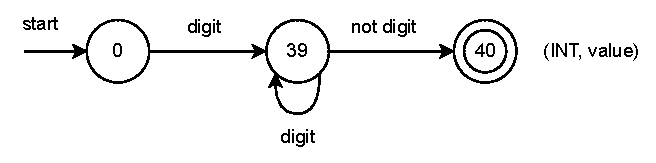
\includegraphics[width=0.9\textwidth]{structures/lexical_analyzer/dps_int.pdf}
	\caption{Диаграмма переходов для определения целого числа}
	\label{f:dps_int}
\end{figure}

При получении в начальном состоянии цифры, выполняется переход в состояние 39, в котором автомат находится до тех пор,
пока не получит на вход символ, отличный от цифры, при получении такого символа выполняется переход в конечное состояние 40.
По мере определения очередной цифры, она заносится в буфер.
В состоянии 40 возвращается токен INT и значение числа из буфера.

Считывание ключевых слов и идентификаторов показано с помощью диаграммы передов на рисунке~\ref{f:dps_ident_kw}.

Из начального состояния происходит переход в состояние 35, если была получена буква.
По аналогии с состоянием 39 выполняется циклическое считывание букв с занесением в буфер.
Если была получена не буква, выполняется переход в состояние 36, в котором проверяется принадлежность считанной строки к списку ключевых слов.
В случае, если считанная строка является ключевым словом, автомат переходит в завершающее состояние 37 в котором указывается тип токена для полученного ключевого слова и значение.
Если в состоянии 36 проверка показала, что строка на является ключевым словом, то выполняется переход в состояние 38 – определен идентификатор.

\begin{figure}[ht]
	\centering
	\vspace{\toppaddingoffigure}
	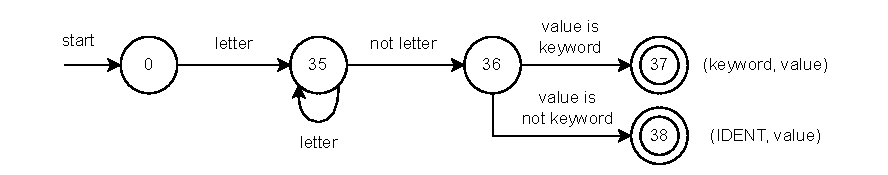
\includegraphics[width=0.9\textwidth]{structures/lexical_analyzer/dps_ident_kw.pdf}
	\caption{Диаграмма переходов для определения идентификаторов и ключевых слов}
	\label{f:dps_ident_kw}
\end{figure}

Полная диаграмма переходов состояний представлена на рисунке~\ref{f:full_dps}

Процесс распознавания токена начинается с начального состояния 0.
В зависимости от полученного символа выполняется переход в конкретное состояние.
Однако, если в начальном состоянии был получен символ, для которого нет дуги,
по которой он бы мог перейти в определенное для него состояние, выполняется переход по дуге «other» в состояние 42 с определением токена ILLEGAL.
После определения очередного токена в конечном состоянии, автомат начинает работу заново с начального состояния.
Считывание входного потока символов прекращается при поступлении нулевого символа (null character) с определением токена EOF.
Вместе с токеном, лексический анализатор возвращает его позицию в входном коде.

% В данном разделе была выполнена разработка структурных решений и алгоритмов функционирования лексического анализатора предметно-ориентированного языка.

\clearpage

\begin{figure}[h!]
	\centering
	\vspace{\toppaddingoffigure}
	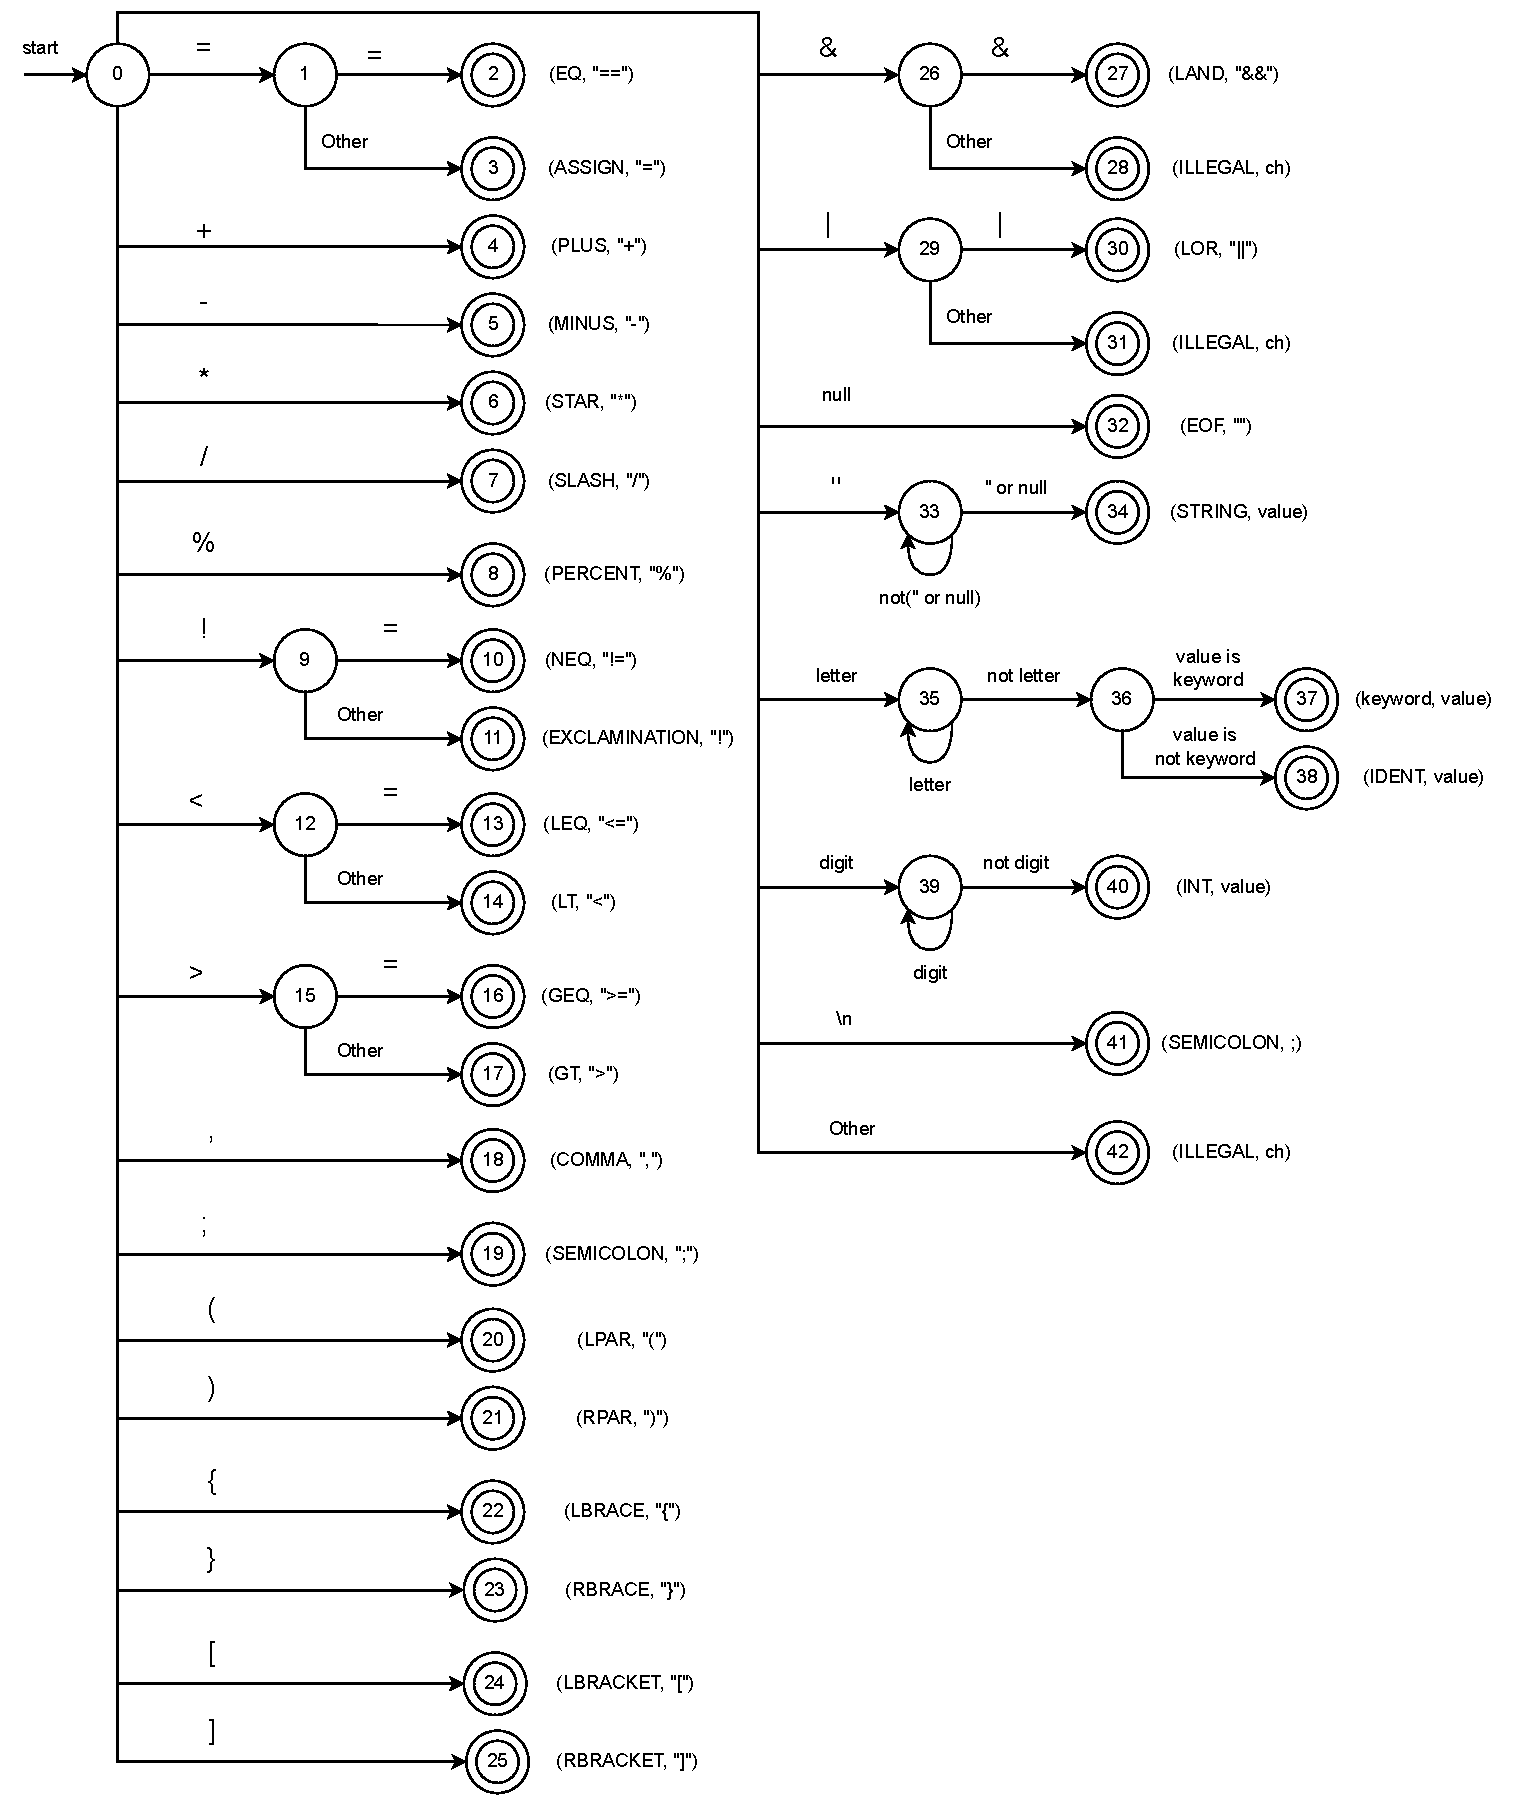
\includegraphics[width=1.0\textwidth]{structures/lexical_analyzer/full_dps.pdf}
	\caption{Полная диаграмма переходов состояний}
	\label{f:full_dps}
\end{figure}

\clearpage
\subsection{Разработка синтаксического анализатора}

% В данном разделе необходимо выполнить разработку алгоритмов функционирования синтаксического анализатора.

Синтаксический анализ – процесс сопоставления последовательности токенов с формальной грамматикой языка.
Результатом работы синтаксического анализатора является абстрактное синтаксическое дерево (AST),
которое отражает синтаксическую структуру входной последовательности и содержит всю необходимую информацию для дальнейших этапов работы транслятора.

В задачу синтаксического анализа входит поиск и выделение основных синтаксических конструкций текста входной программы,
установление типа и проверка правильности каждой синтаксической конструкции, а так же представление их в виде AST.

Существует два основных метода синтаксического анализа:

\begin{itemize}
    \item нисходящий;
    \item восходящий.
\end{itemize}

В данном проекте реализован нисходящий анализатор, работающий по методу рекурсивного спуска,
известный как парсер Пратта, который впервые описал Вон Пратт в статье «Нисходящий парсер с операторным предшествованием».

Этот метод основан на идее приоритета операторов и обработке различных уровней приоритета в выражениях.
В парсере Пратта каждый оператор имеет свой уровень приоритета.
Операторы с более высоким приоритетом связываются с операндами сильнее, чем операторы с более низким приоритетом.
Значения приоритетов для каждого оператора разрабатываемого предметно-ориентированного языка показаны в таблице~\ref{t:operator_priority}.

\clearpage

\begin{table}[h!]
    \Large
    \caption{Приоритеты операторов}
    \label{t:operator_priority}
    \centering
    \begin{tabularx}{\textwidth}{|c|X|}
        \hline
        Приоритет & Операторы             \\
        \hline
        0         & Минимальный приоритет \\
        \hline
        1         & =                     \\
        \hline
        2         & | |                   \\
        \hline
        3         & \&\&                  \\
        \hline
        4         & == !=                 \\
        \hline
        5         & < > <= >=             \\
        \hline
        6         & + -                   \\
        \hline
        7         & * / \%                \\
        \hline
        8         & -x or !x              \\
        \hline
        9         & (                     \\
        \hline
        10        & [                     \\
        \hline
    \end{tabularx}
    \vspace{\bottompaddingoftable}
\end{table}

Для примера работы приоритета операторов рассмотрим пример построения AST для арифметического выражения: $3 + 1 * 4 * 6 + 8$.
Диаграмма, показывающая рекурсивные вызовы для формирования выражений к приведенному примеру изображена на рисунке~\ref{f:priorities}.

\begin{figure}[ht]
	\centering
	\vspace{\toppaddingoffigure}
	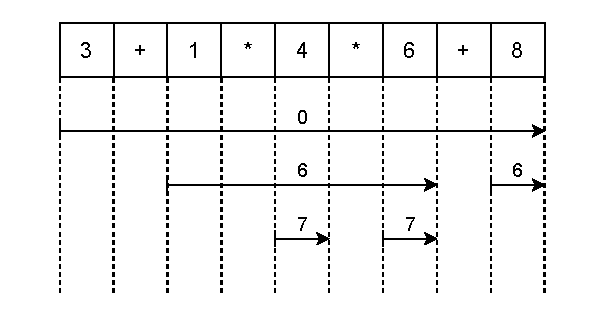
\includegraphics[width=0.7\textwidth]{structures/parser/priorities.pdf}
	\caption{Диаграмма рекурсивных вызовов}
	\label{f:priorities}
\end{figure}

Над стрелками обозначены приоритеты операторов, к которым относится эта стрелка.
В самом начале распознавания выражения значение приоритета равняется 0.
По мере обнаружения оператора, приоритет которого выше текущего алгоритм переходит на следующий уровень рекурсии.
По диаграмме видно, что справа от первого оператора «+» длинная стрелка с приоритетом 6, группирует члены умножения, так как операция умножения имеет больший приоритет, чем сложение.
Эта стрелка заканчивается перед последним «+», так как приоритет оператора, относящегося к этой стрелке не ниже приоритета последнего «+».
Другими словами, экземпляр выражения с более низким приоритетом ожидает результата формирования выражения с более высоким приоритетом.

Абстрактное синтаксическое дерево для данного примера приведено на рисунке~\ref{f:ast_example}.

\begin{figure}[ht]
	\centering
	\vspace{\toppaddingoffigure}
	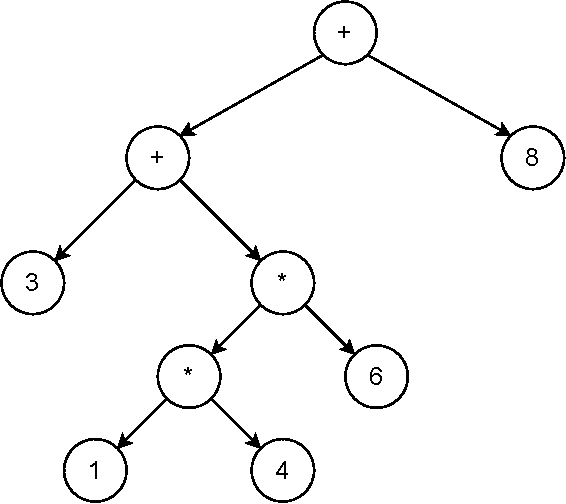
\includegraphics[width=0.7\textwidth]{structures/parser/ast_example.pdf}
	\caption{Абстрактное синтаксическое дерево}
	\label{f:ast_example}
\end{figure}

Некоторые схемы алгоритма построения абстрактного синтаксического дерева представлены на рисунках~\ref{f:parse_program}~-~\ref{f:parse_Expression}.

% В данном разделе была выполнена разработка структурных решений и алгоритмов функционирования синтаксического анализатора.

\clearpage

\begin{figure}[!htp]
	\centering
	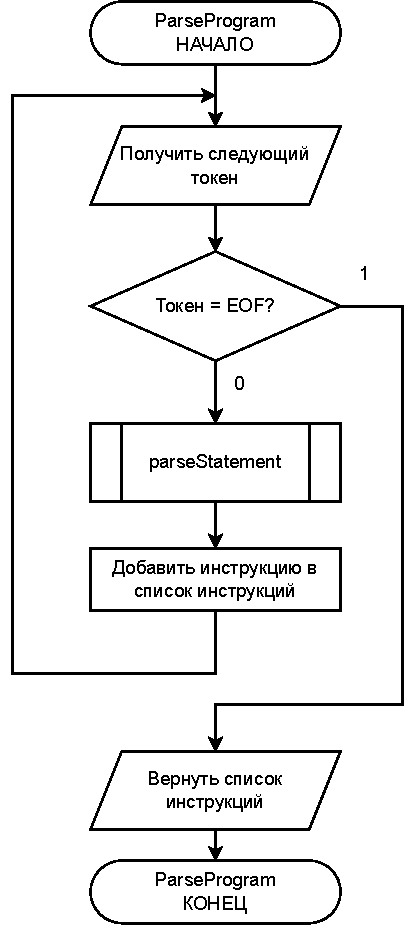
\includegraphics[width=0.5\textwidth]{structures/parser/parse_program.pdf}
	\caption{Схема алгоритма «ParseProgram»}
	\label{f:parse_program}
\end{figure}

\clearpage

\begin{figure}[!htp]
	\centering
	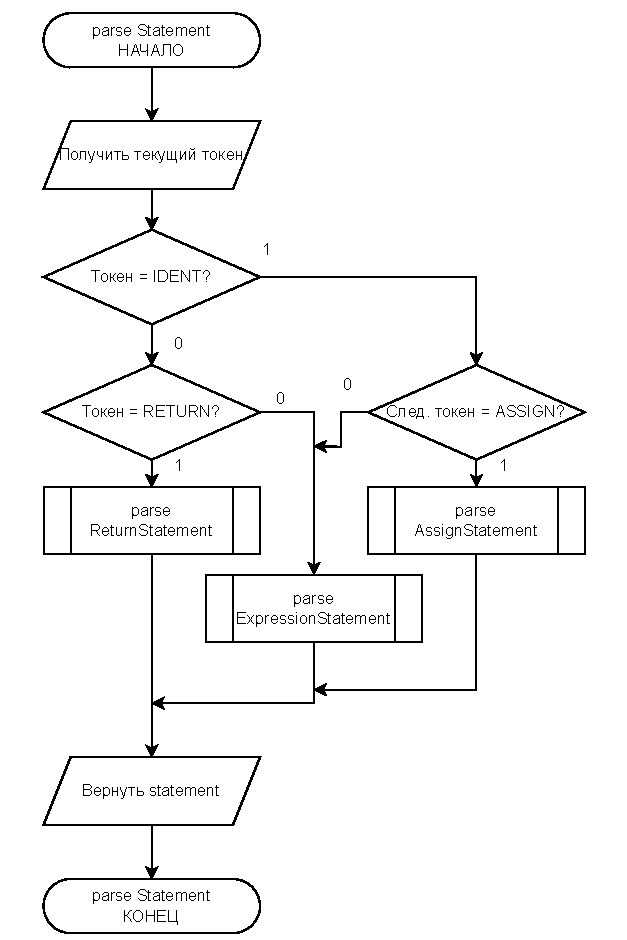
\includegraphics[width=0.7\textwidth]{structures/parser/parse_statement.pdf}
	\caption{Схема алгоритма «parseStatement»}
	\label{f:parse_statement}
\end{figure}

\clearpage

\begin{figure}[!htp]
	\centering
	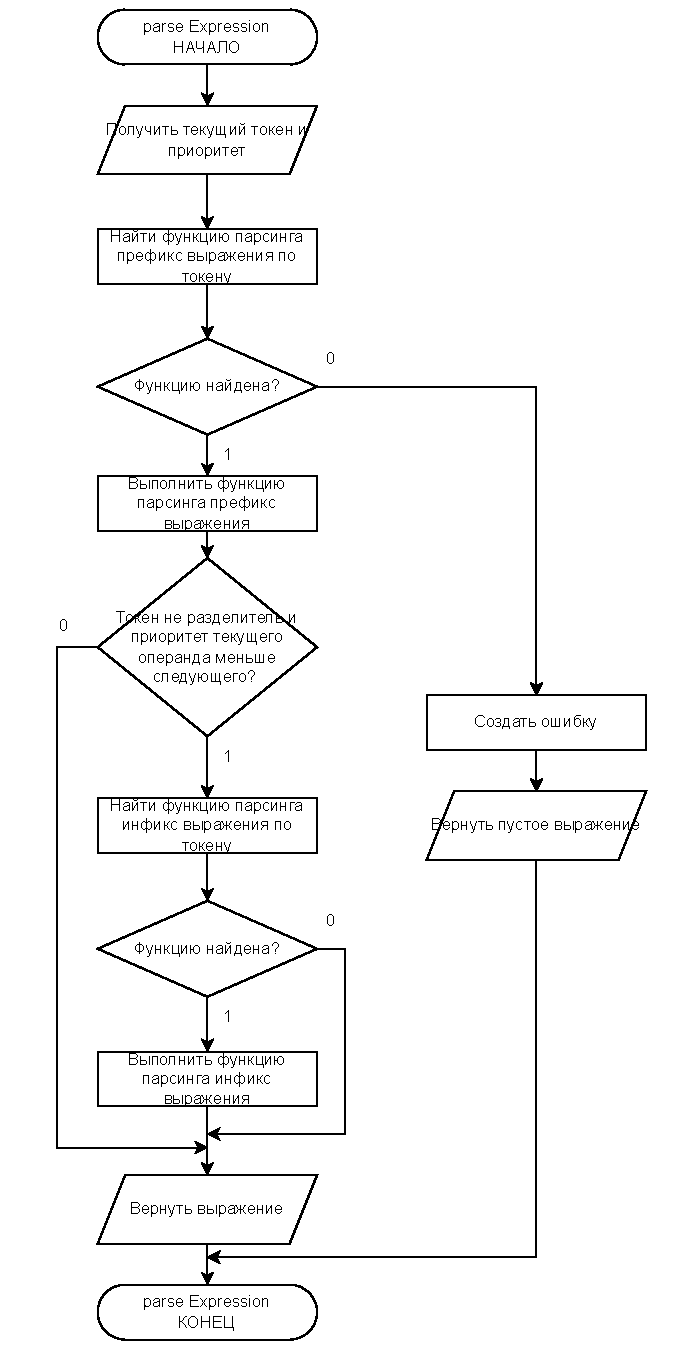
\includegraphics[width=0.60\textwidth]{structures/parser/parse_Expression.pdf}
	\caption{Схема алгоритма «parseExpression»}
	\label{f:parse_Expression}
\end{figure}

\clearpage


\subsection{Разработка семантического анализатора}

% В данном разделе необходимо выполнить разработку алгоритмов функционирования семантического анализатора.

Семантический анализ – это этап работы транслятора, вот время которого выполняется проверка текста исходной программы с точки зрения семантики языка.
В ходе семантического анализа выполняется такие операции, как проверка типов данных, правильность использования переменных, функций, выражений, а также обнаружение смысловых ошибок в коде.

Обобщенная модульная структура серверной части конструктора представлена на рисунке~\ref{f:modules_server_struct}.

Процесс семантического анализа выполняется после построения абстрактного синтаксического дерева синтаксическим анализатором.
Семантический анализ сгруппирован с этапом исполнения выражений.
Таким образом при одном проходе AST алгоритм выполняет проверку узла дерева на семантическую корректность и переход к его исполнению,
если не было обнаружено ошибок при семантическим анализе. В случае обнаружения семантической ошибки возвращается информация о ней,
а процесс интерпретации переход к следующему выражению.

На этапе проектирования семантического анализатора закладываются решения, которые лягут в основу принципов написания кода на разрабатываемом языке.
Например, на этапе построения семантического анализатора, нужно решить, как будет обрабатываться значение в условном выражении, не имеющее тип boolean.
Есть несколько вариантов обработки таких значений.
Один из них - всегда принимать данное значение за «false» и идти в соответствующую ветвь.
В ином случае, при обнаружении значения с типом, отличным от boolean необходимо вернуть ошибку и прекратить выполнение данного выражения.
В этом проекте будет использован второй вариант с возвратом ошибки.

Семантический анализатор принимает на вход элементы абстрактного синтаксического дерева.
После проверки семантической корректности выражения AST, следует его вычисление.
Результаты вычислений выражений, как промежуточные, так и окончательные необходимо каким-то образом представить в памяти.
Это необходимо в первую очередь для получения ранее вычисленных выражений и работы с ними.
В качестве примера можно рассмотреть код, представленный на рисунке~\ref{f:code_example_var}.

\begin{figure}[ht]
	\centering
	\vspace{\toppaddingoffigure}
	\begin{lstlisting}
X = 5;
X + 3
\end{lstlisting}
	\caption{Пример кода использования объявленной переменной}
	\label{f:code_example_var}
\end{figure}

В первой строке присваивается значение 5 переменной «X».
Затем выполняется выражение «X + 3».
Чтобы получить значение данного выражения нужно получить ранее вычисленное значение 5.
Для этого необходимо как-то сохранить его в памяти.

Решение данной задачи состоит в введении внутреннего представления вычисленных значений на время семантического анализа и этапа исполнения.
Примем некоторую объектную систему, состоящую из набора объектов, каждый из которых будет содержать информацию о представляемом им типе данных в предметно-ориентированном языке.

Каждый объект должен содержать информацию о значении представляемого им типа данных предметно-ориентированного языка.
Кроме этого, необходимо реализовать возможность определения того, какой тип данных предметно-ориентированного языка представляет объект, а также функционал получения строкового значения объекта.
Кроме этого, типы данных: целое число, строка и булево значение могут использоваться в виде ключей в хэш-карте.
Для этого необходимо специально для объектов, представляющих эти типы предусмотреть функцию вычисления хэш строки от их значения. 

Объектная система должна представлять все типы данных предметно-ориентированного языка, а именно:
целые числа, строки, булевы значения, массивы, хэш-карты.
Также необходимо ввести дополнительные объекты, представляющие семантические ошибки, значение «null», функции, операцию возврата значения из функции.

Объектная система может быть представлена в виде диаграммы классов.
Диаграмма классов представлена на рисунке~\ref{f:class_diagram}.

\clearpage

\begin{figure}[!htp]
	\centering
    \vspace{\toppaddingoffigure}
	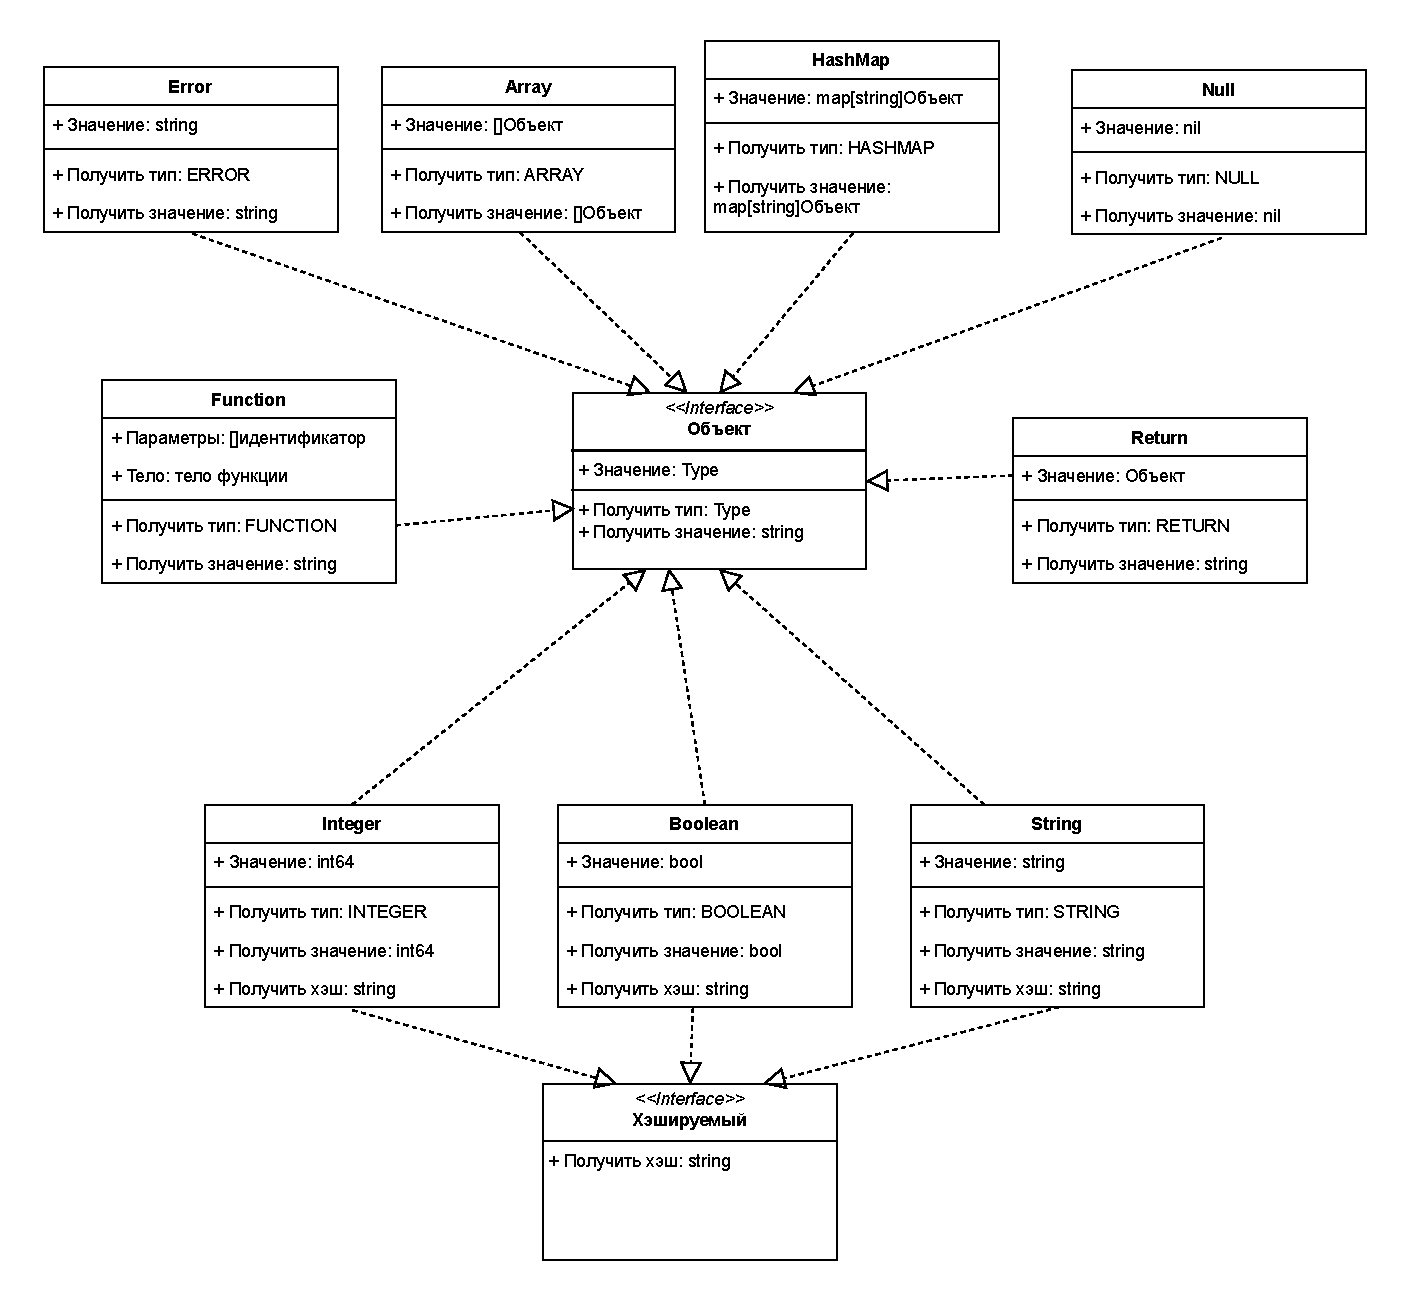
\includegraphics[width=1.0\textwidth]{structures/semantic_analyzer/class_diagram.pdf}
	\caption{Диаграмма классов}
	\label{f:class_diagram}
\end{figure}

В качестве примера работы алгоритма на рисунках~\ref{f:evalProgram}~-~\ref{f:semantic_index_expr} приведены схемы алгоритмов семантического анализа некоторых выражений.

% В данном разделе была выполнена разработка структурных решений и алгоритмов функционирования семантического анализатора.

\begin{figure}[!htp]
	\centering
	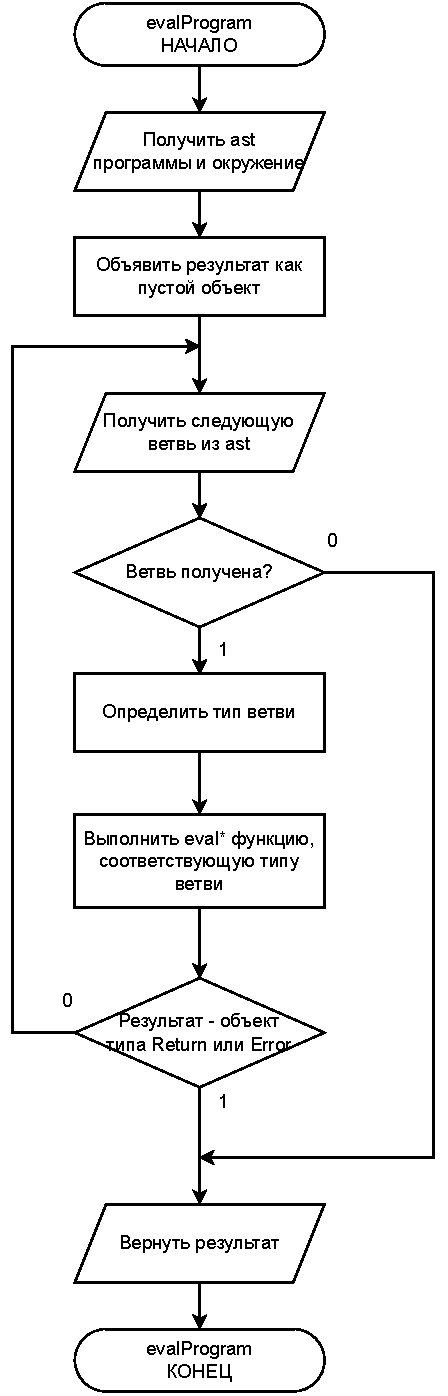
\includegraphics[width=0.4\textwidth]{structures/semantic_analyzer/semantic_Program.pdf}
	\caption{Схема алгоритма «evalProgram»}
	\label{f:evalProgram}
\end{figure}

\clearpage

\begin{figure}[!htp]
	\centering
	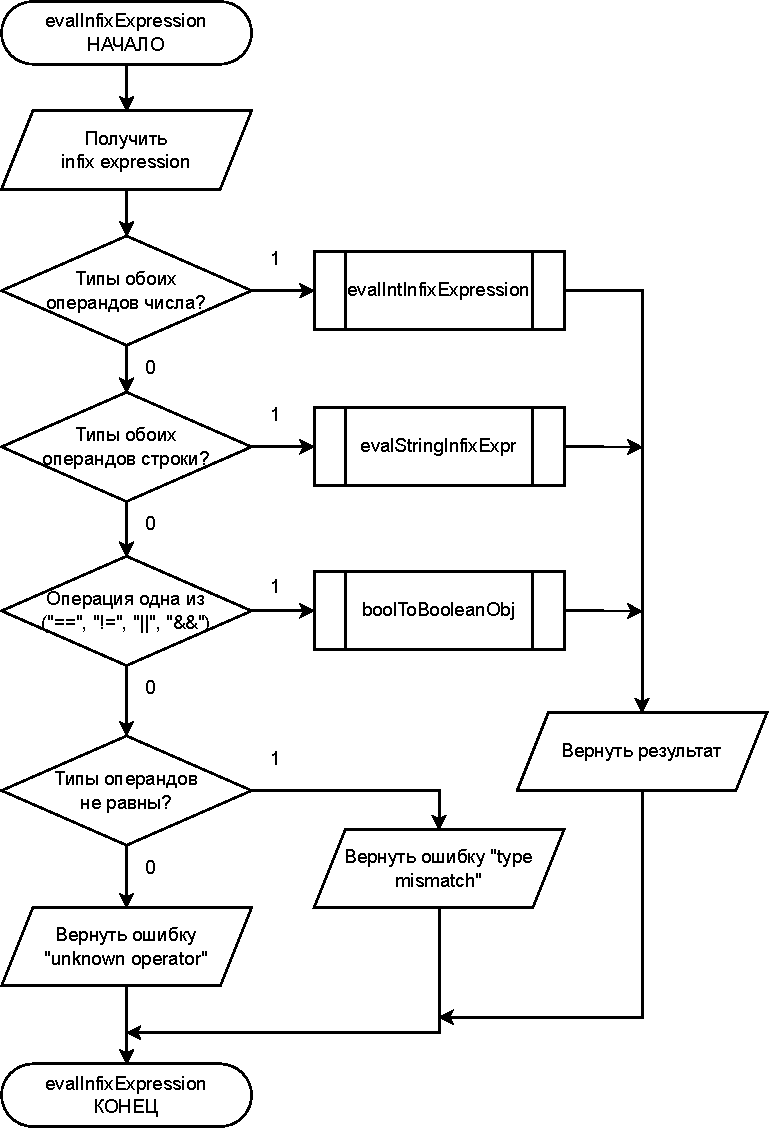
\includegraphics[width=0.9\textwidth]{structures/semantic_analyzer/semantic_infix_expr.pdf}
	\caption{Схема алгоритма «evalInfixExpression»}
	\label{f:semantic_infix_expr}
\end{figure}

\clearpage

\begin{figure}[!htp]
	\centering
	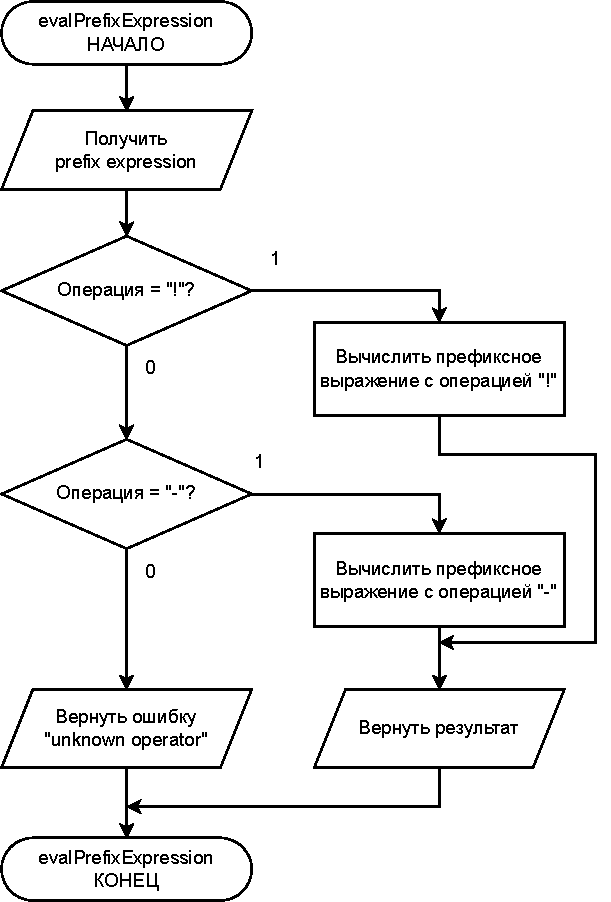
\includegraphics[width=0.9\textwidth]{structures/semantic_analyzer/semantic_prefix_expr.pdf}
	\caption{Схема алгоритма «evalPrefixExpression»}
	\label{f:semantic_prefix_expr}
\end{figure}

\clearpage

\begin{figure}[!htp]
	\centering
	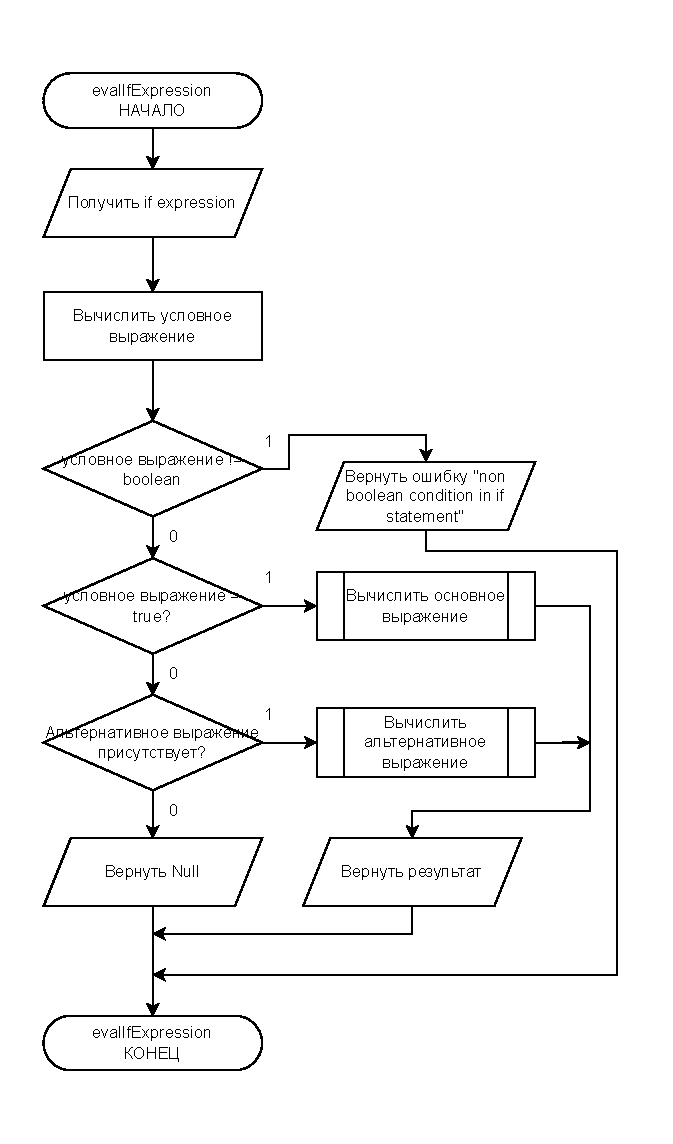
\includegraphics[width=0.7\textwidth]{structures/semantic_analyzer/semantic_if_expr.pdf}
	\caption{Схема алгоритма «evalIfExpression»}
	\label{f:semantic_if_expr}
\end{figure}

\clearpage

\begin{figure}[!htp]
	\centering
	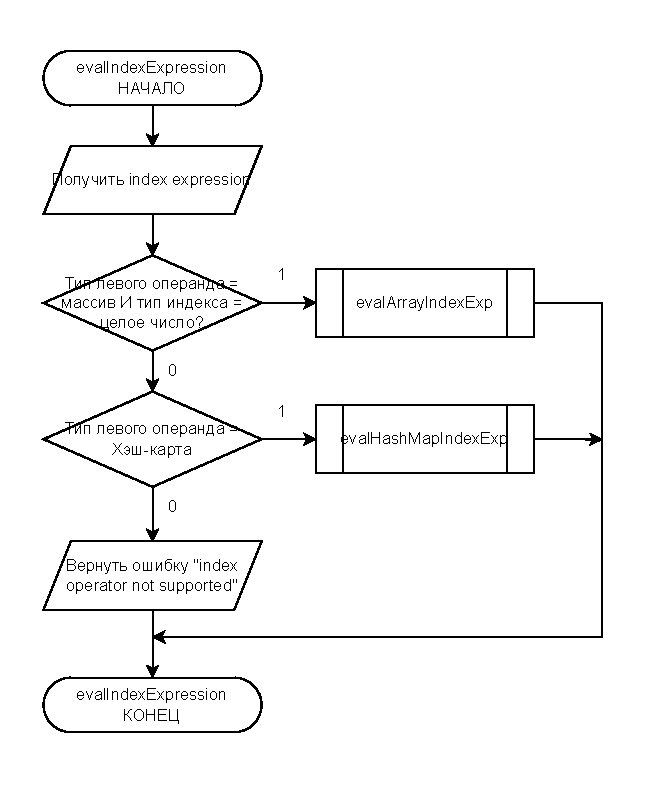
\includegraphics[width=0.75\textwidth]{structures/semantic_analyzer/semantic_index_expr.pdf}
	\caption{Схема алгоритма «evalIndexExpression»}
	\label{f:semantic_index_expr}
\end{figure}
\subsection{Разработка исполнителя}

Процесс вычисления выполняется над выражениями из узлов абстрактного синтаксического дерева.
Такой вид интерпретатора, который работает с AST называется <<tree walking interpreter>> или древовидный интерпретатор.
В таком интерпретаторе выполняется обход AST и выполнение соответствующих операций для каждого узла.

Последним этапом в процессе обработки исходного кода является его исполнение.
До этого шага все выражения языка представляют собой набор символов, токенов или ветви абстрактного синтаксического дерева без какого-либо семантического значения.
На данном этапе выражения языка приобретают смысл, то есть начинают интерпретироваться и действовать в соответствии с правилами и инструкциями языка.

Этап исполнения выполняется непосредственно после семантического анализа.
Если во время семантического анализа в обрабатываемом выражении не было обнаружено ошибок, выполняется переход к его вычислению.
Вычисление выражения выполняется в зависимости от его типа, например,
для инфиксного выражения применяется указанная в нем операция над левым и правым операндами и формируется результат в виде объекта соответствующего типа,
содержащего результат операции, а для условного выражения сначала вычисляется значение условия,
а затем в зависимости от его результата выполняется либо основная ветвь (при значении условия «true»), либо альтернативная (при значении условия «false»).

Только лишь вычислять значения выражений недостаточно.
Нужно также сохранять значения переменных для того, чтоб к ним можно было обратиться при обнаружении в выражениях.
Чтобы обеспечить эту возможность введем окружение – структуру данных, хранящую информацию о переменных и связанных с ними значениях на время выполнения программы.
Таким образом, при объявлении переменной, информация о ней будет записываться в окружение, а при необходимости получить значение этой переменой – ее значение будет считано из окружения.

В качестве примера работы алгоритма на рисунках~\ref{f:eval_int_infix_expr}~-~\ref{f:eval_string_infix_expr} приведены схемы алгоритма вычисления некоторых выражений.

\clearpage

\begin{figure}[!htp]
	\centering
	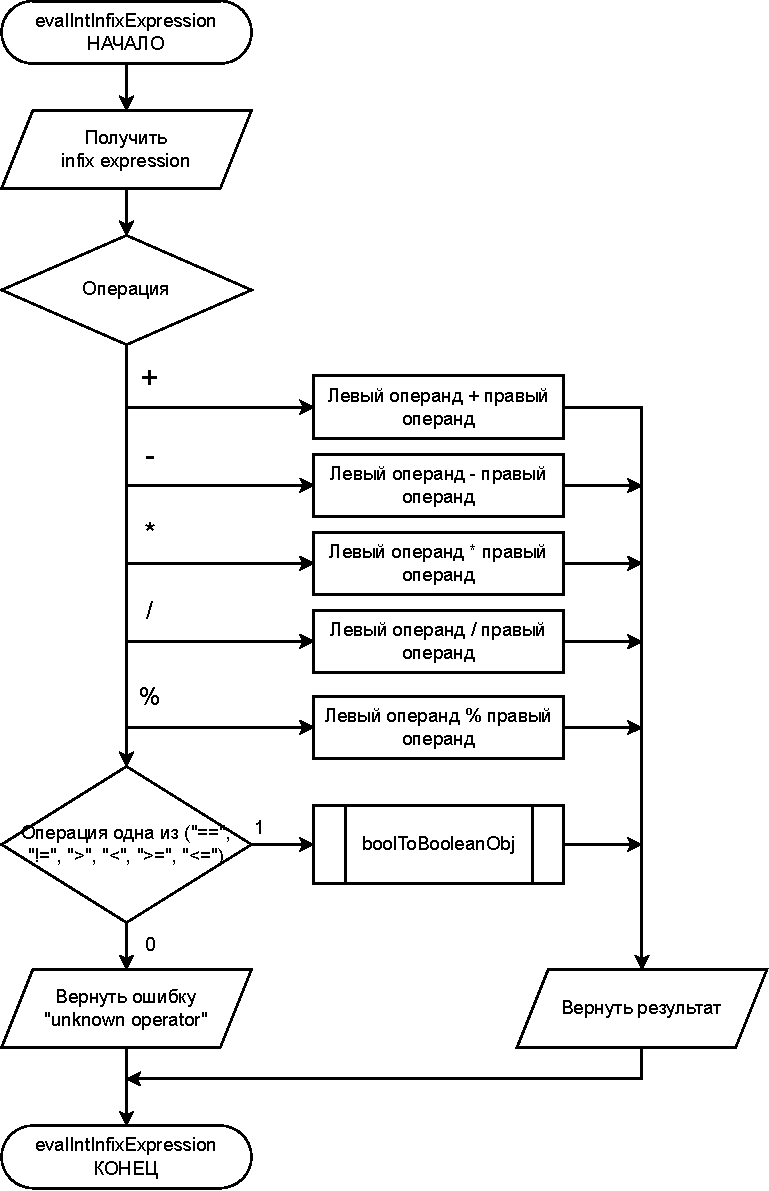
\includegraphics[width=0.8\textwidth]{structures/evaluator/eval_int_infix_expr.pdf}
	\caption{Схема алгоритма вычисления целочисленного инфиксного выражения}
	\label{f:eval_int_infix_expr}
\end{figure}

\clearpage

\begin{figure}[!htp]
	\centering
	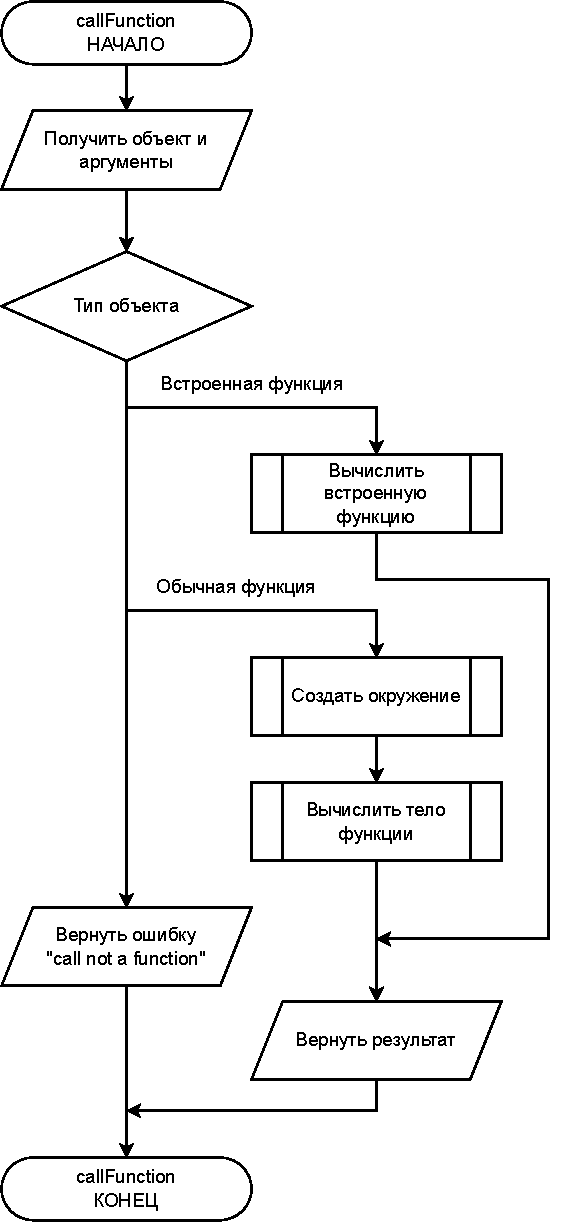
\includegraphics[width=0.6\textwidth]{structures/evaluator/eval_callFunction.pdf}
	\caption{Схема алгоритма исполнения вызова функции}
	\label{f:eval_callFunction}
\end{figure}

\clearpage

\begin{figure}[!htp]
	\centering
	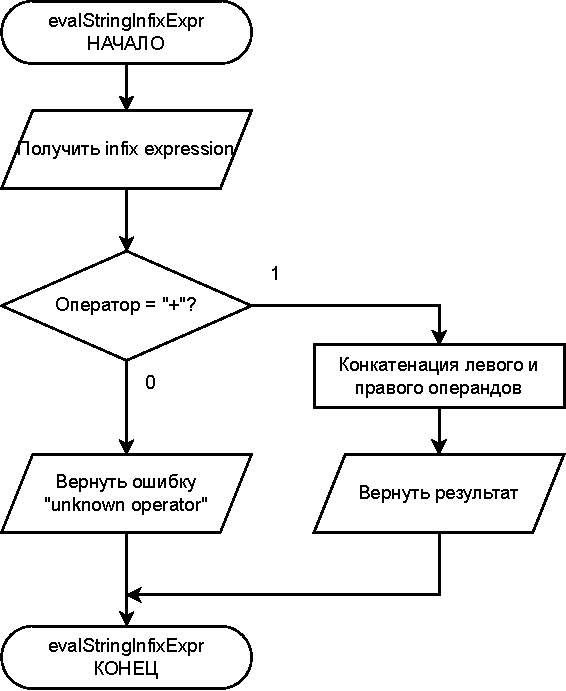
\includegraphics[width=0.5\textwidth]{structures/evaluator/eval_string_infix_expr.pdf}
	\caption{Схема алгоритма вычисления инфиксного выражения для строк}
	\label{f:eval_string_infix_expr}
\end{figure}

\section*{Вывод}

В данном разделе были разработаны архитектурно-структурные решения по поставленной задаче.
Рассмотрена модульная структура серверной части конструктора,
определена связь между модулем компонентов и модулем интерпретации предметно-ориентированного языка.

Рассмотрена обобщенная структура интерпретатора и этапы его работы.

Выполнен обзор способов задания языков, разработана и описана с помощью расширенной формы Бэкуса-Наура формальная грамматика предметно-ориентированного языка.
Выполнена разработка структурных решений и алгоритмов функционирования каждого из этапов интерпретатора, а именно:
лексического анализатора, синтаксического анализатора, семантического анализатора и исполнителя.